\begin{introduction}
The mobile applications usage is growing. The native development of an application for each, individual platform is well used across many companies. However, many of them, predominantly smaller ones, concludes that developing and maintenance of each platform is not cheap and comes with much of work. On the other hand, there are technologies which offer cross-platform development with one code-base. Every cross-platform technology takes its own approach to how the code base is compiled to the native platform. 

Some of them use the concept of bridging the cross-platform user interface primitives to its counterpart in the native platform. Well-known examples are React~Native~\cite{react-native} or Xamarin~Forms~\cite{xamarin-forms}. The opposite approach is the form of a progressive web application (PWA) where the application is written as a web-based application with support of native features. This approach uses, for example, Ionic framework~\cite{ionic}. 

\begin{figure}[htp]
    \centering
    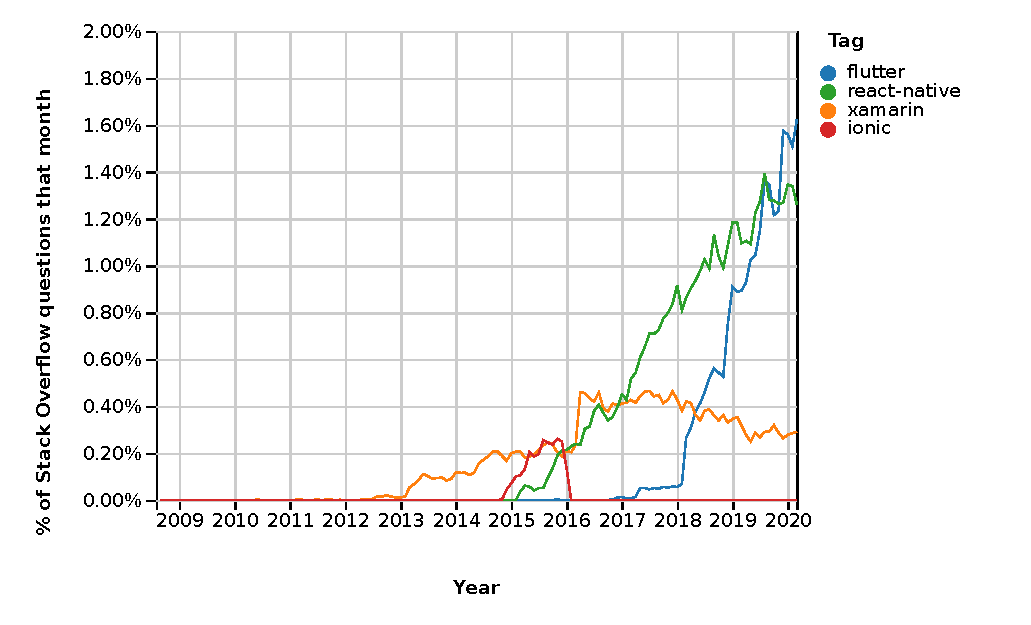
\includegraphics[width=0.9\linewidth]{img/introduction/so-flutter-trend.pdf}
    \caption{Flutter trend against other popular cross-platform frameworks~\cite{so-flutter-trend}}
    \label{fig:so-flutter-trend}
\end{figure}

During 2017, the concept of another approach was proposed, where the application uses low-level platform API to draw over the whole screen with keeping high performance and access to native features. Later on, from this concept open-source framework Flutter, made by Google,  was created~\cite{flutter}. 

The Flutter for the last three years until now (first half of 2020) started to gain developers attention, and it was highly promoted by Google. One indication of its growing popularity is \textit{Stack~Overflow Developer Survey~2019}~\cite{so-2019-survey} where it took third place of ``Most Loved'' framework directly after \textit{.NET Core} and \textit{Torch/PyTorch} and highly growing trend among questions created during the last years (see \Cref{fig:so-flutter-trend}). However, like with every new technology, the Flutter can become well-known and well used or will be left as a dead-end. 

\section{Motivation}
There are many reasons why the author chose this topic for the thesis. First of all, his bachelor thesis~\cite{nymsap-bp} already focused on mobile application development, although it used different cross-platform technology -- Xamarin. During his ongoing studies, the author discovered and started to use new, by his opinion, promising framework Flutter. So his first goal and motivation was to study Flutter more in-depth and bring comprehensive study material of this framework for others. The second reason was to conclude if Flutter can become a framework which can be used to create production-ready applications or if it is still an experimental framework. Last reason was motivation to create complex, and yet, simple to use mobile application for everyone who seeks to find new cafes to visit.

\section{Structure}
The thesis is divided to four chapters:
\begin{itemize}
\item \Cref{ch:flutter} deals with introduction to Flutter framework, its concept and internal functionality.
\item \Cref{ch:analysis} introduce proposed Coffee Time application. Describes the created prototype and its user testing. The analysis of back-end services is described. 
\item \Cref{ch:implementation} describes process of back-end implementation as well of Coffee Time application. In the chapter, details how its implemented, which approaches was taken and how development process was done. 
\item \Cref{ch:testing} describes final application release and its testing. 
\end{itemize}
In conclusion, the results are compared with the goals of this thesis. 
\end{introduction}